\chapter{Конструкторская часть}
\textbf{Требования к вводу:}
\begin{enumerate}
  	\item на вход подаются две строки;
	\item прописные и строчные буквы считаются разными.
\end{enumerate}
\textbf{Требования к программе:}
\begin{enumerate}
  	\item две пустые строки - корректный ввод, программа не должна аварийно завершаться;
  	\item программа должна уметь обрабатывать слова на русском языке.
\end{enumerate}
\section{Схемы алгоритмов}
В данной части будут рассмотрены схемы алгоритмов.

\begin{figure}[h]
\centering
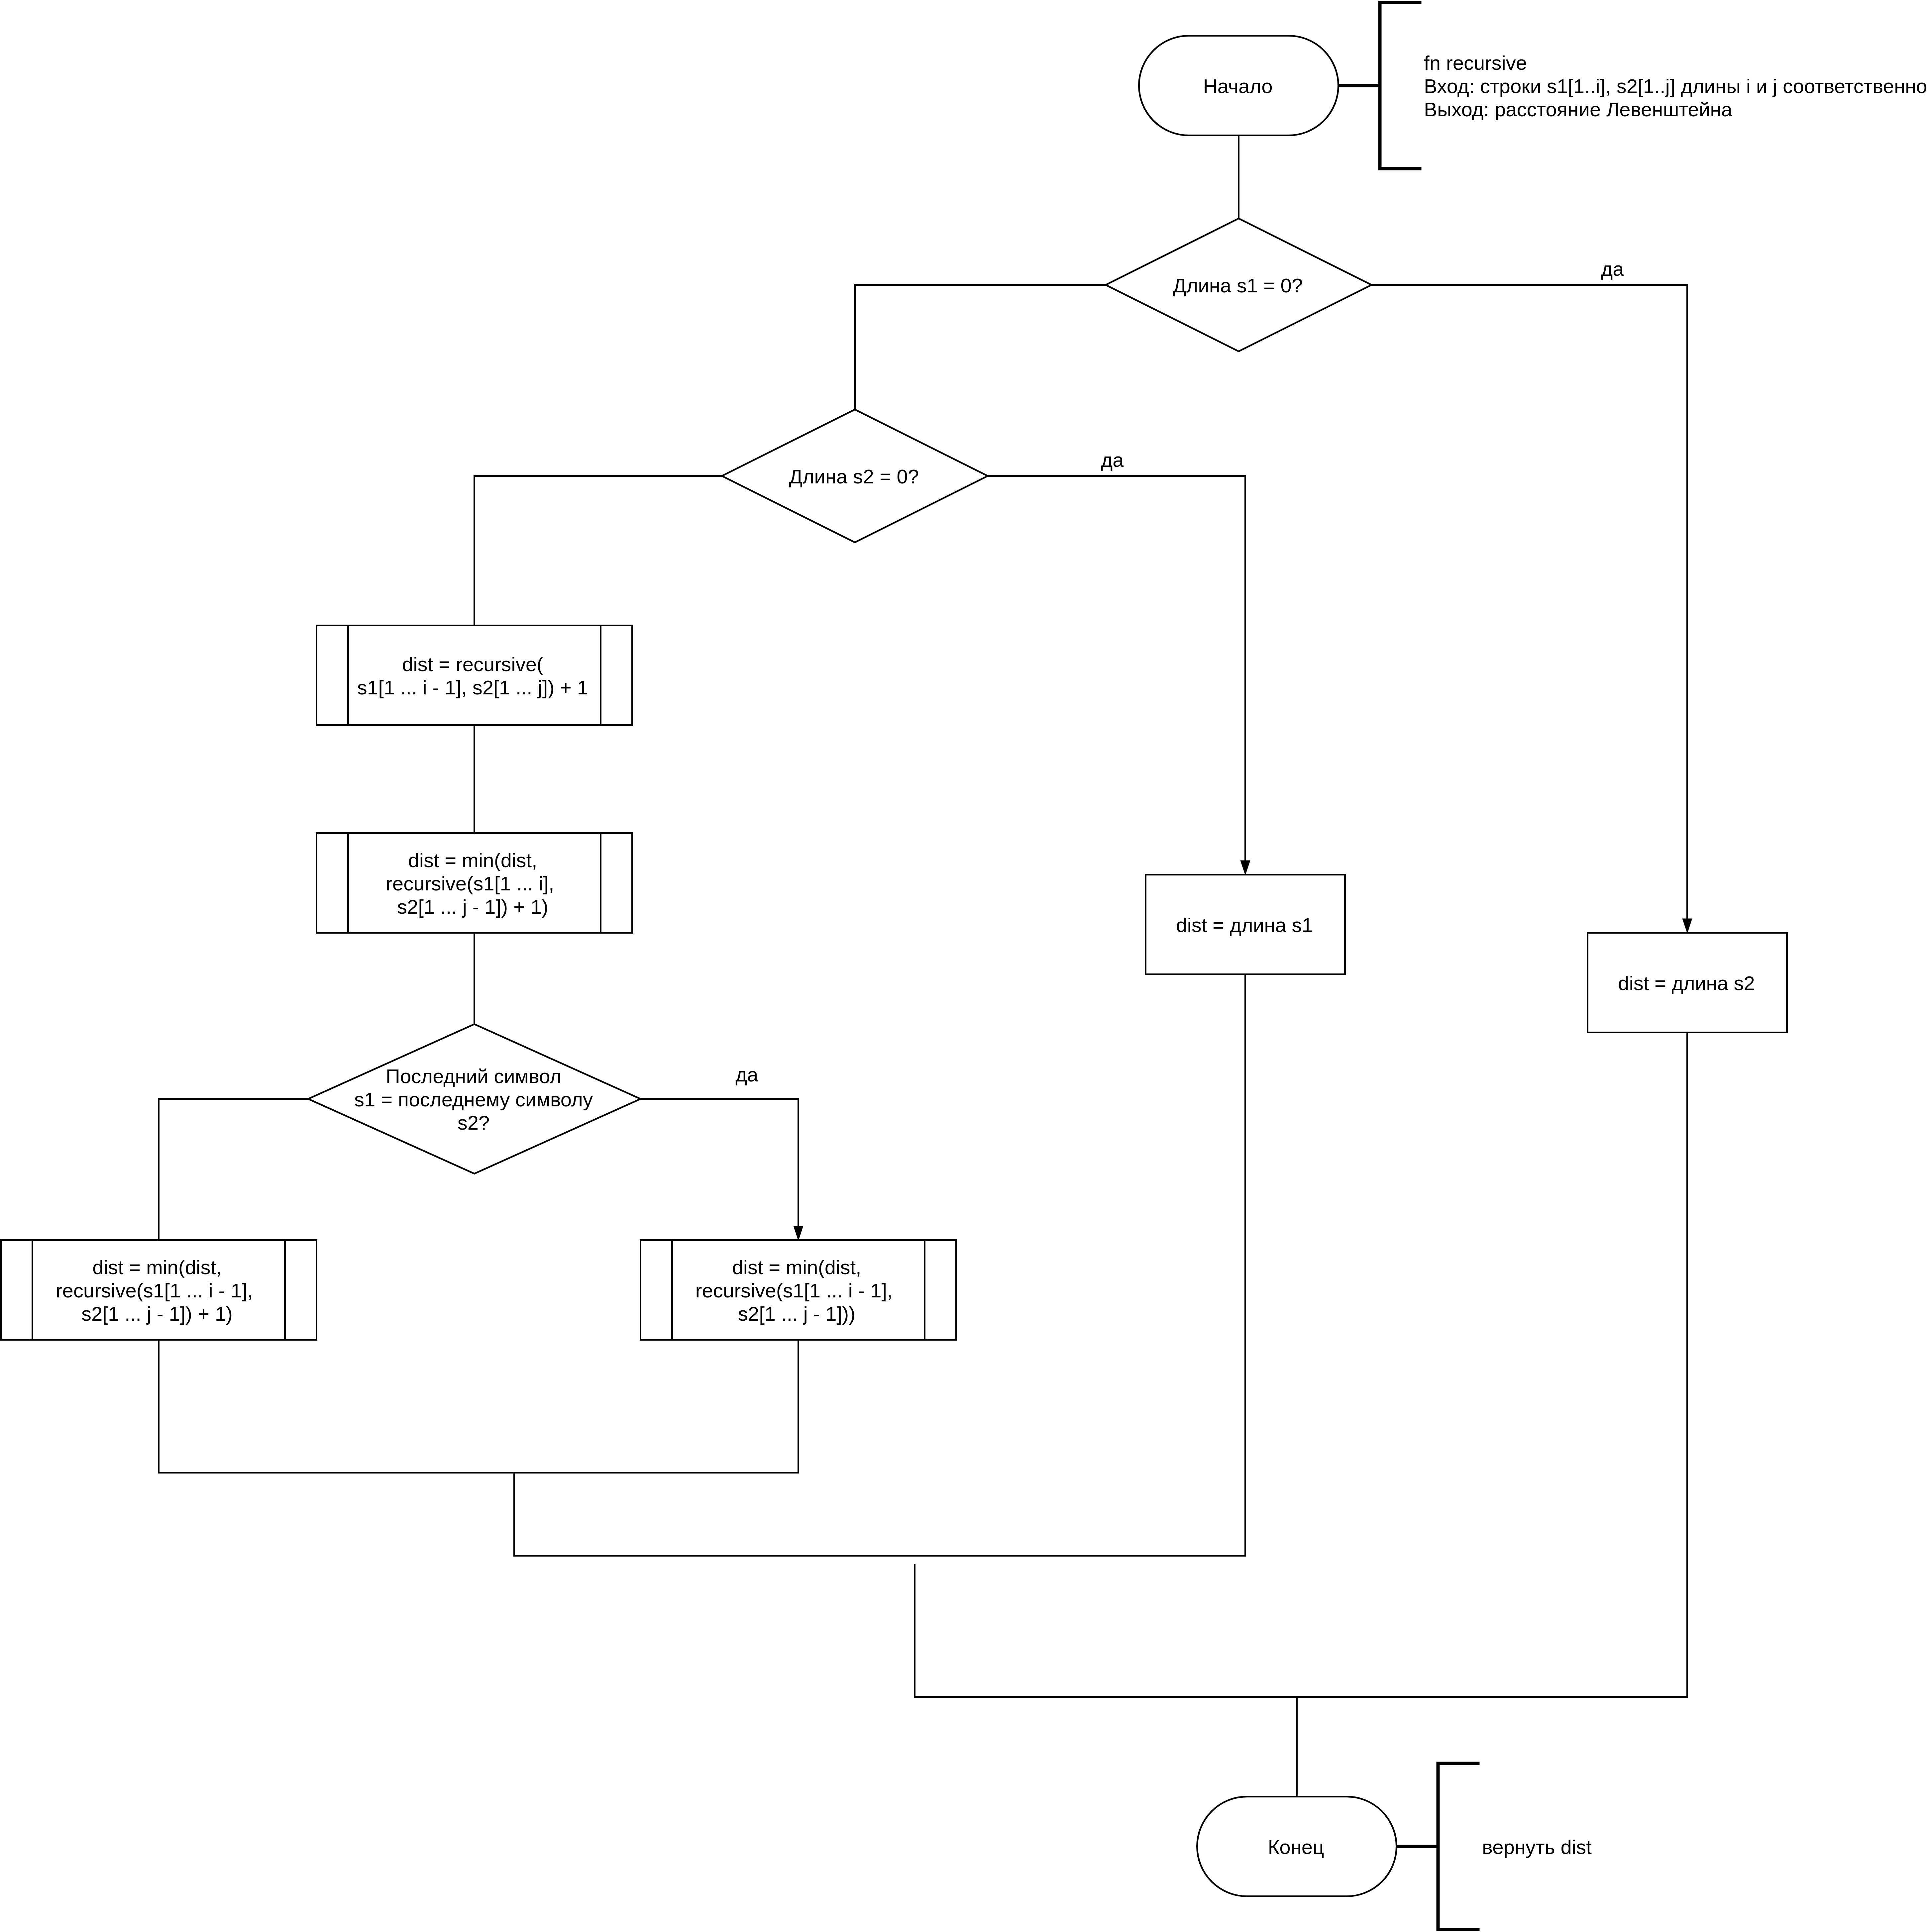
\includegraphics[width=180mm]{recursive}
\caption{Схема рекурсивного алгоритма нахождения расстояния Левенштейна}
\label{fig:mpr}
\end{figure}

\begin{figure}[h]
\centering
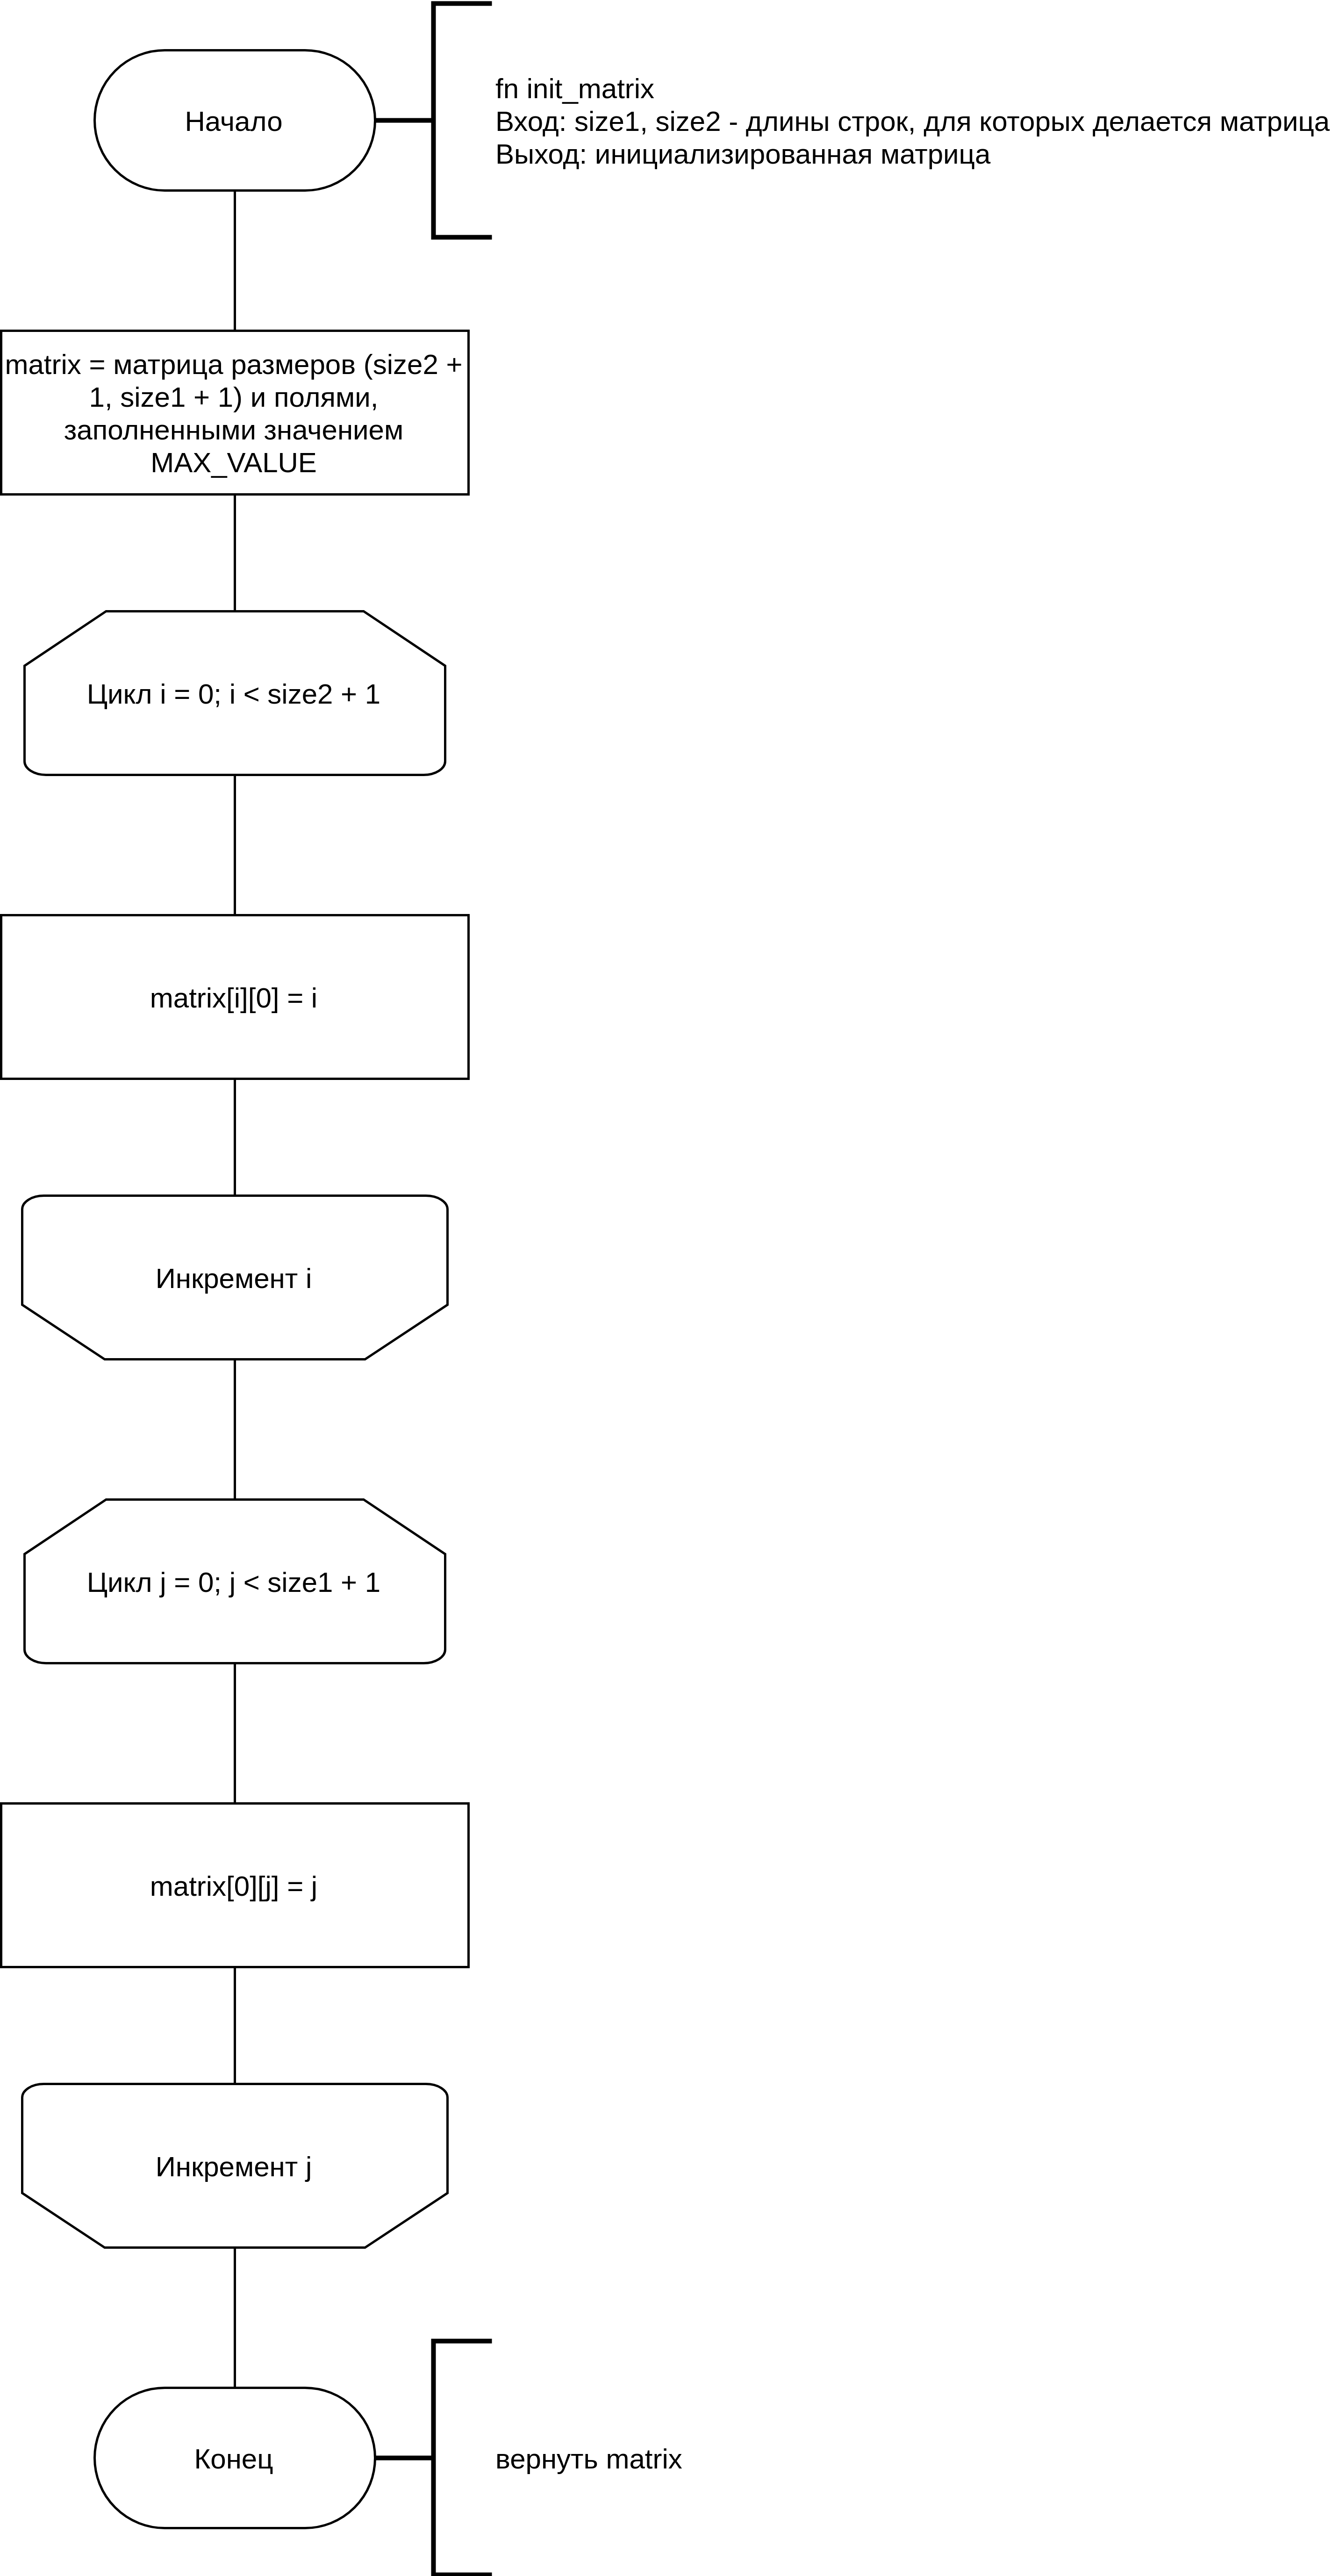
\includegraphics[height=180mm]{init_matrix}
\caption{Схема алгоритма инициализации матрицы для итеративных и рекурсивного с мемоизацией алгоритмов}
\label{fig:mpr}
\end{figure}

\begin{figure}[h]
\centering
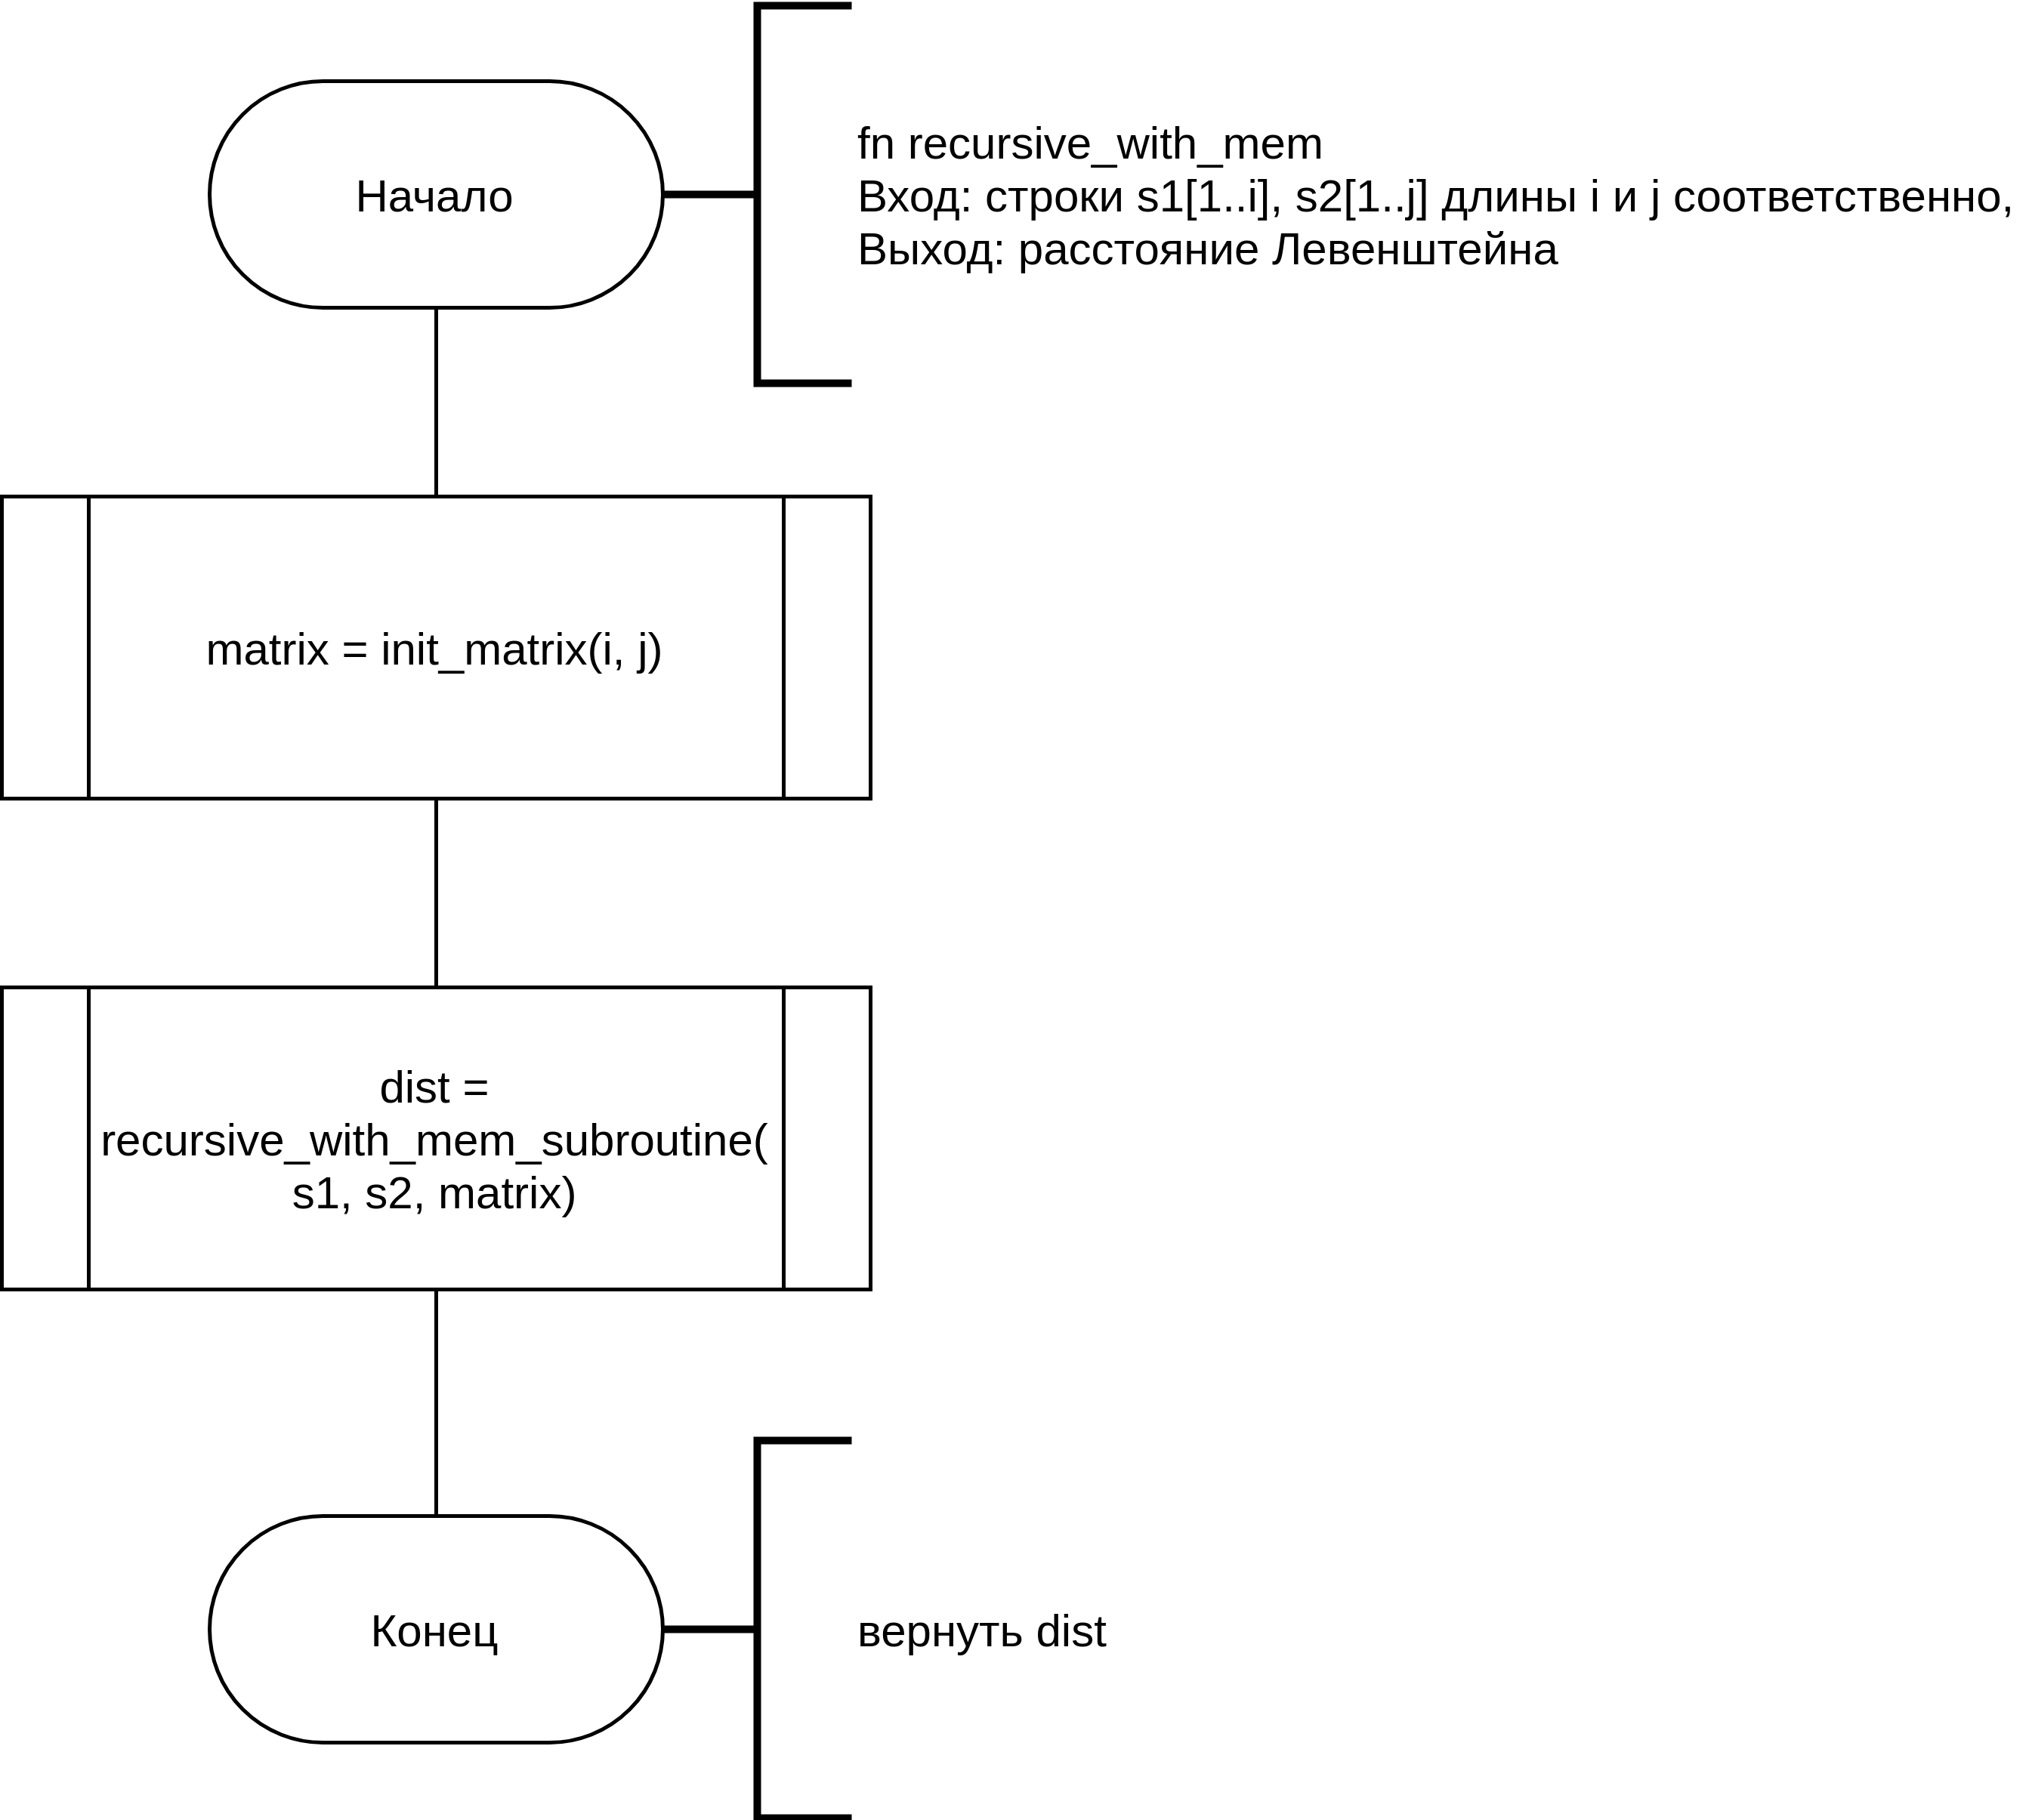
\includegraphics[height=120mm]{rec_mem}
\caption{Схема рекурсивного алгоритма с мемоизацией нахождения расстояния Левенштейна}
\label{fig:mpr}
\end{figure}

\begin{figure}[h]
\centering
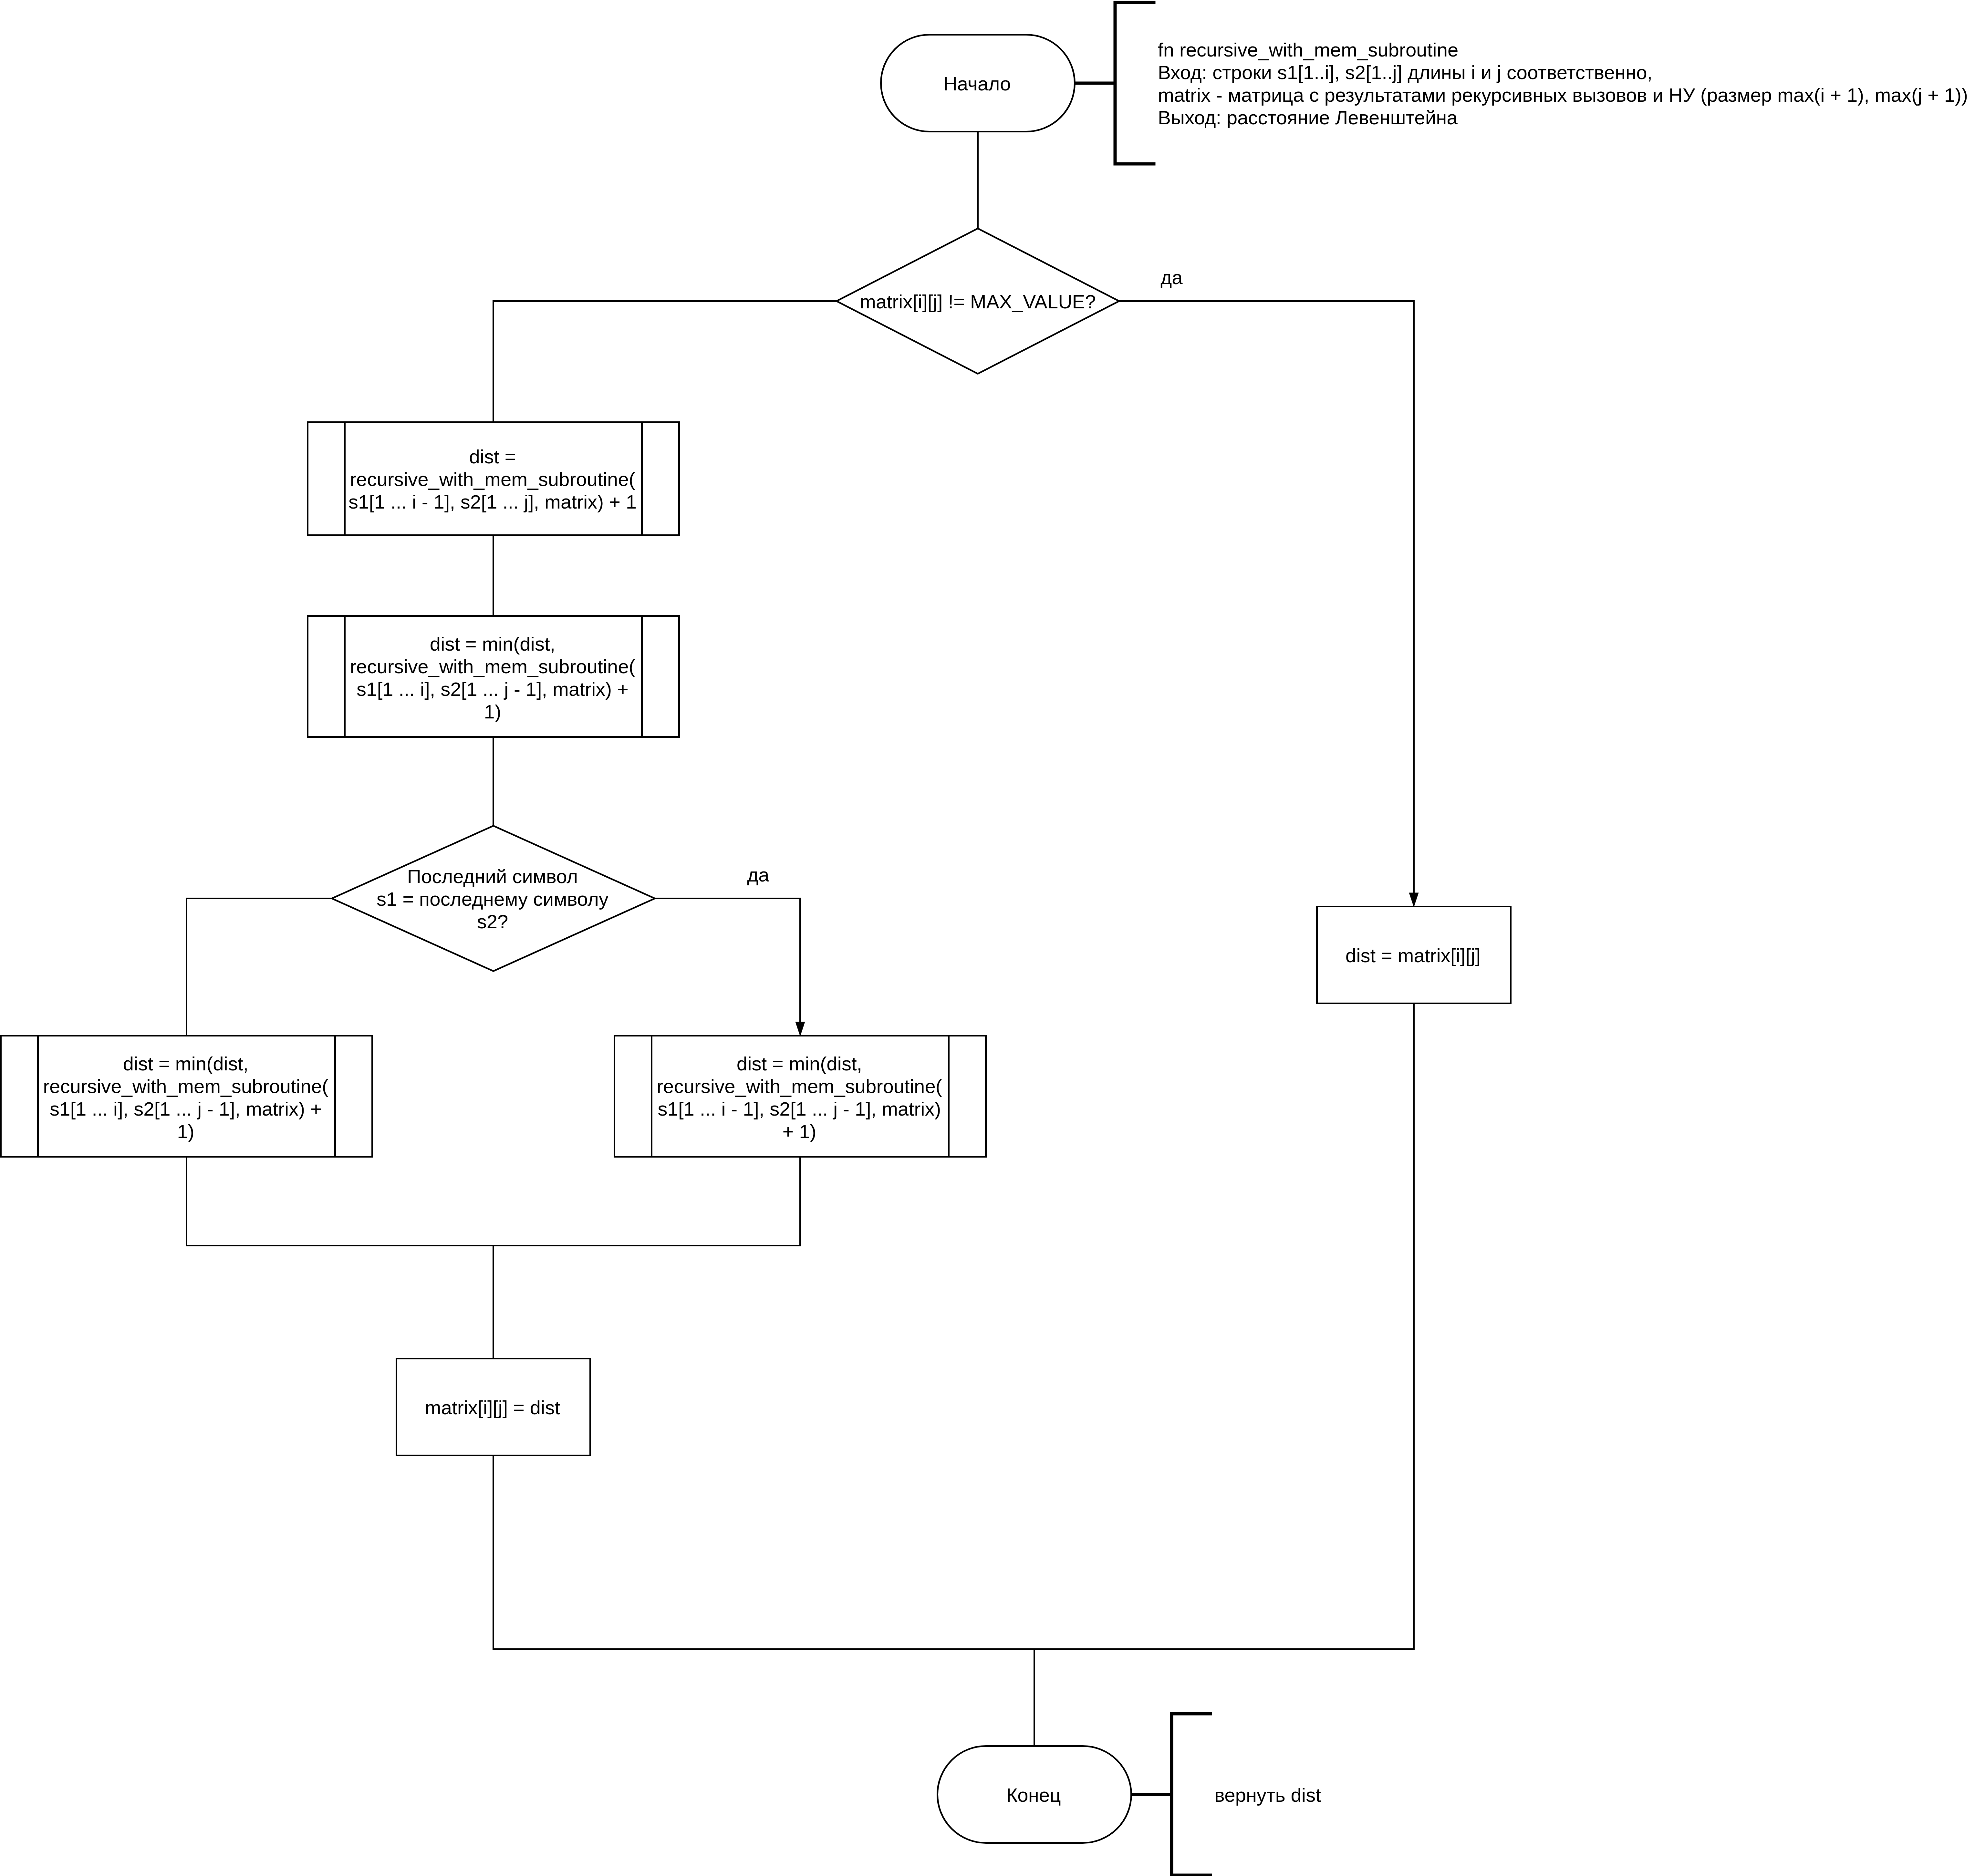
\includegraphics[width=180mm]{recursive_with_mem}
\caption{Схема процедуры рекурсивного алгоритма с мемоизацией нахождения расстояния Дамерау-Левенштейна}
\label{fig:mpr}
\end{figure}

\begin{figure}[h]
\centering
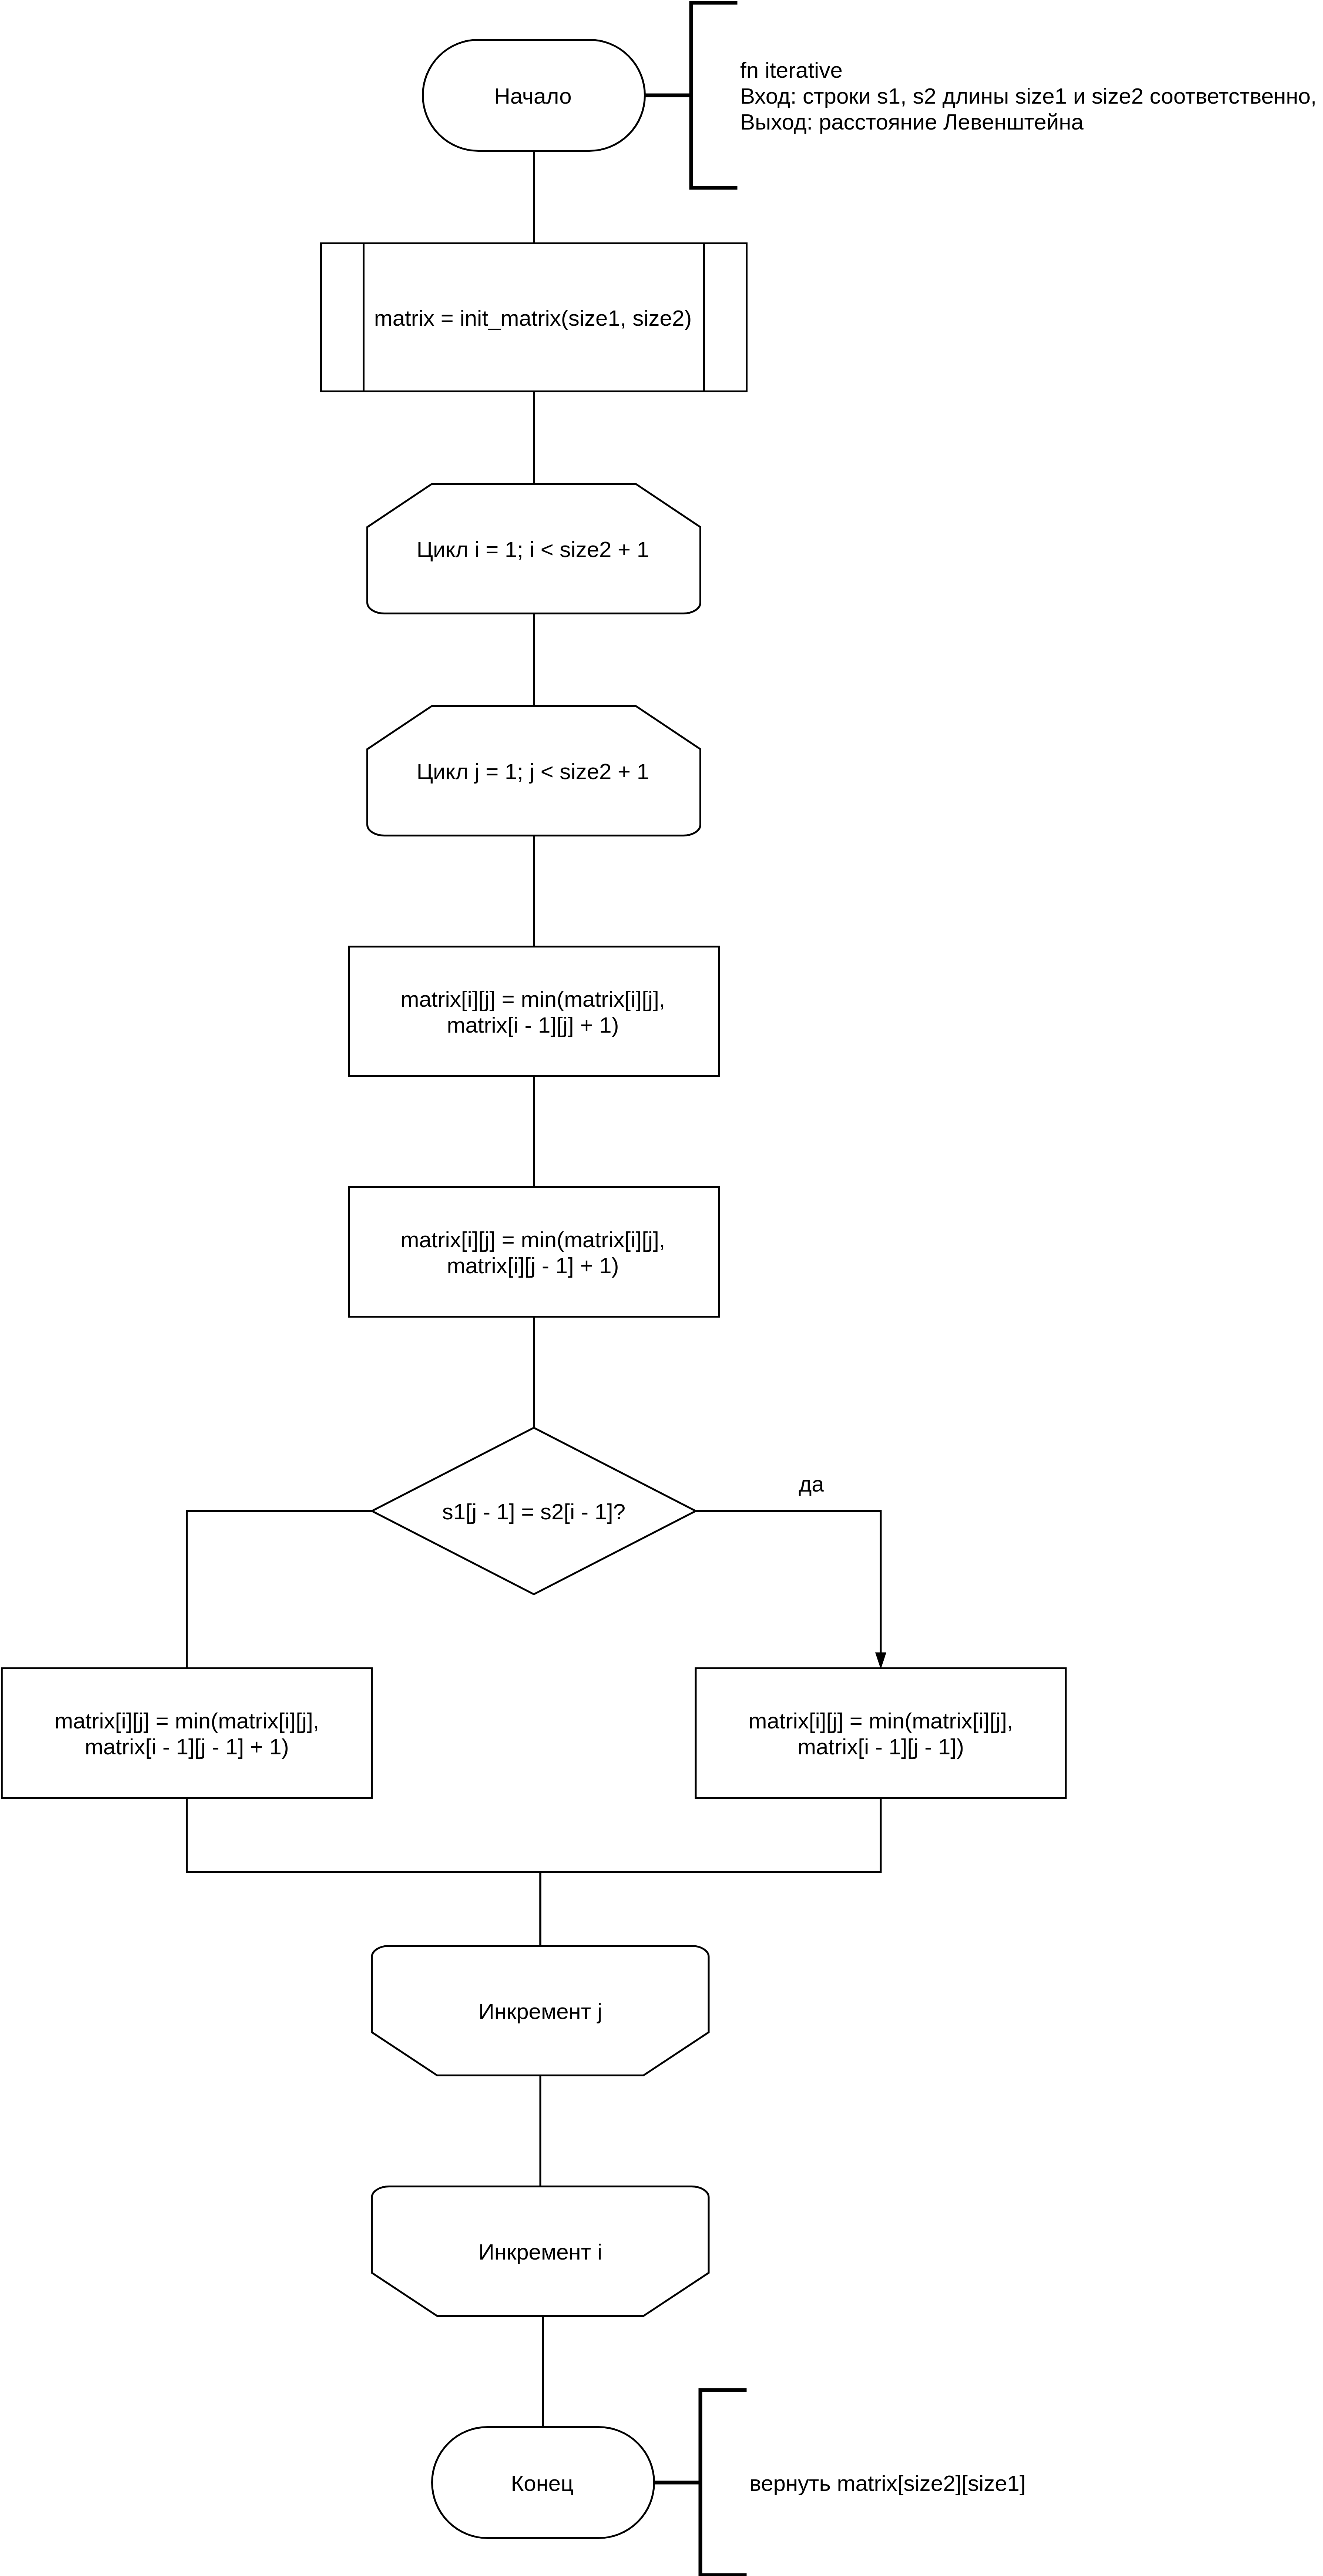
\includegraphics[height=220mm]{iterative}
\caption{Схема итеративного алгоритма нахождения расстояния Левенштейна}
\label{fig:mpr}
\end{figure}

\begin{figure}[h]
\centering
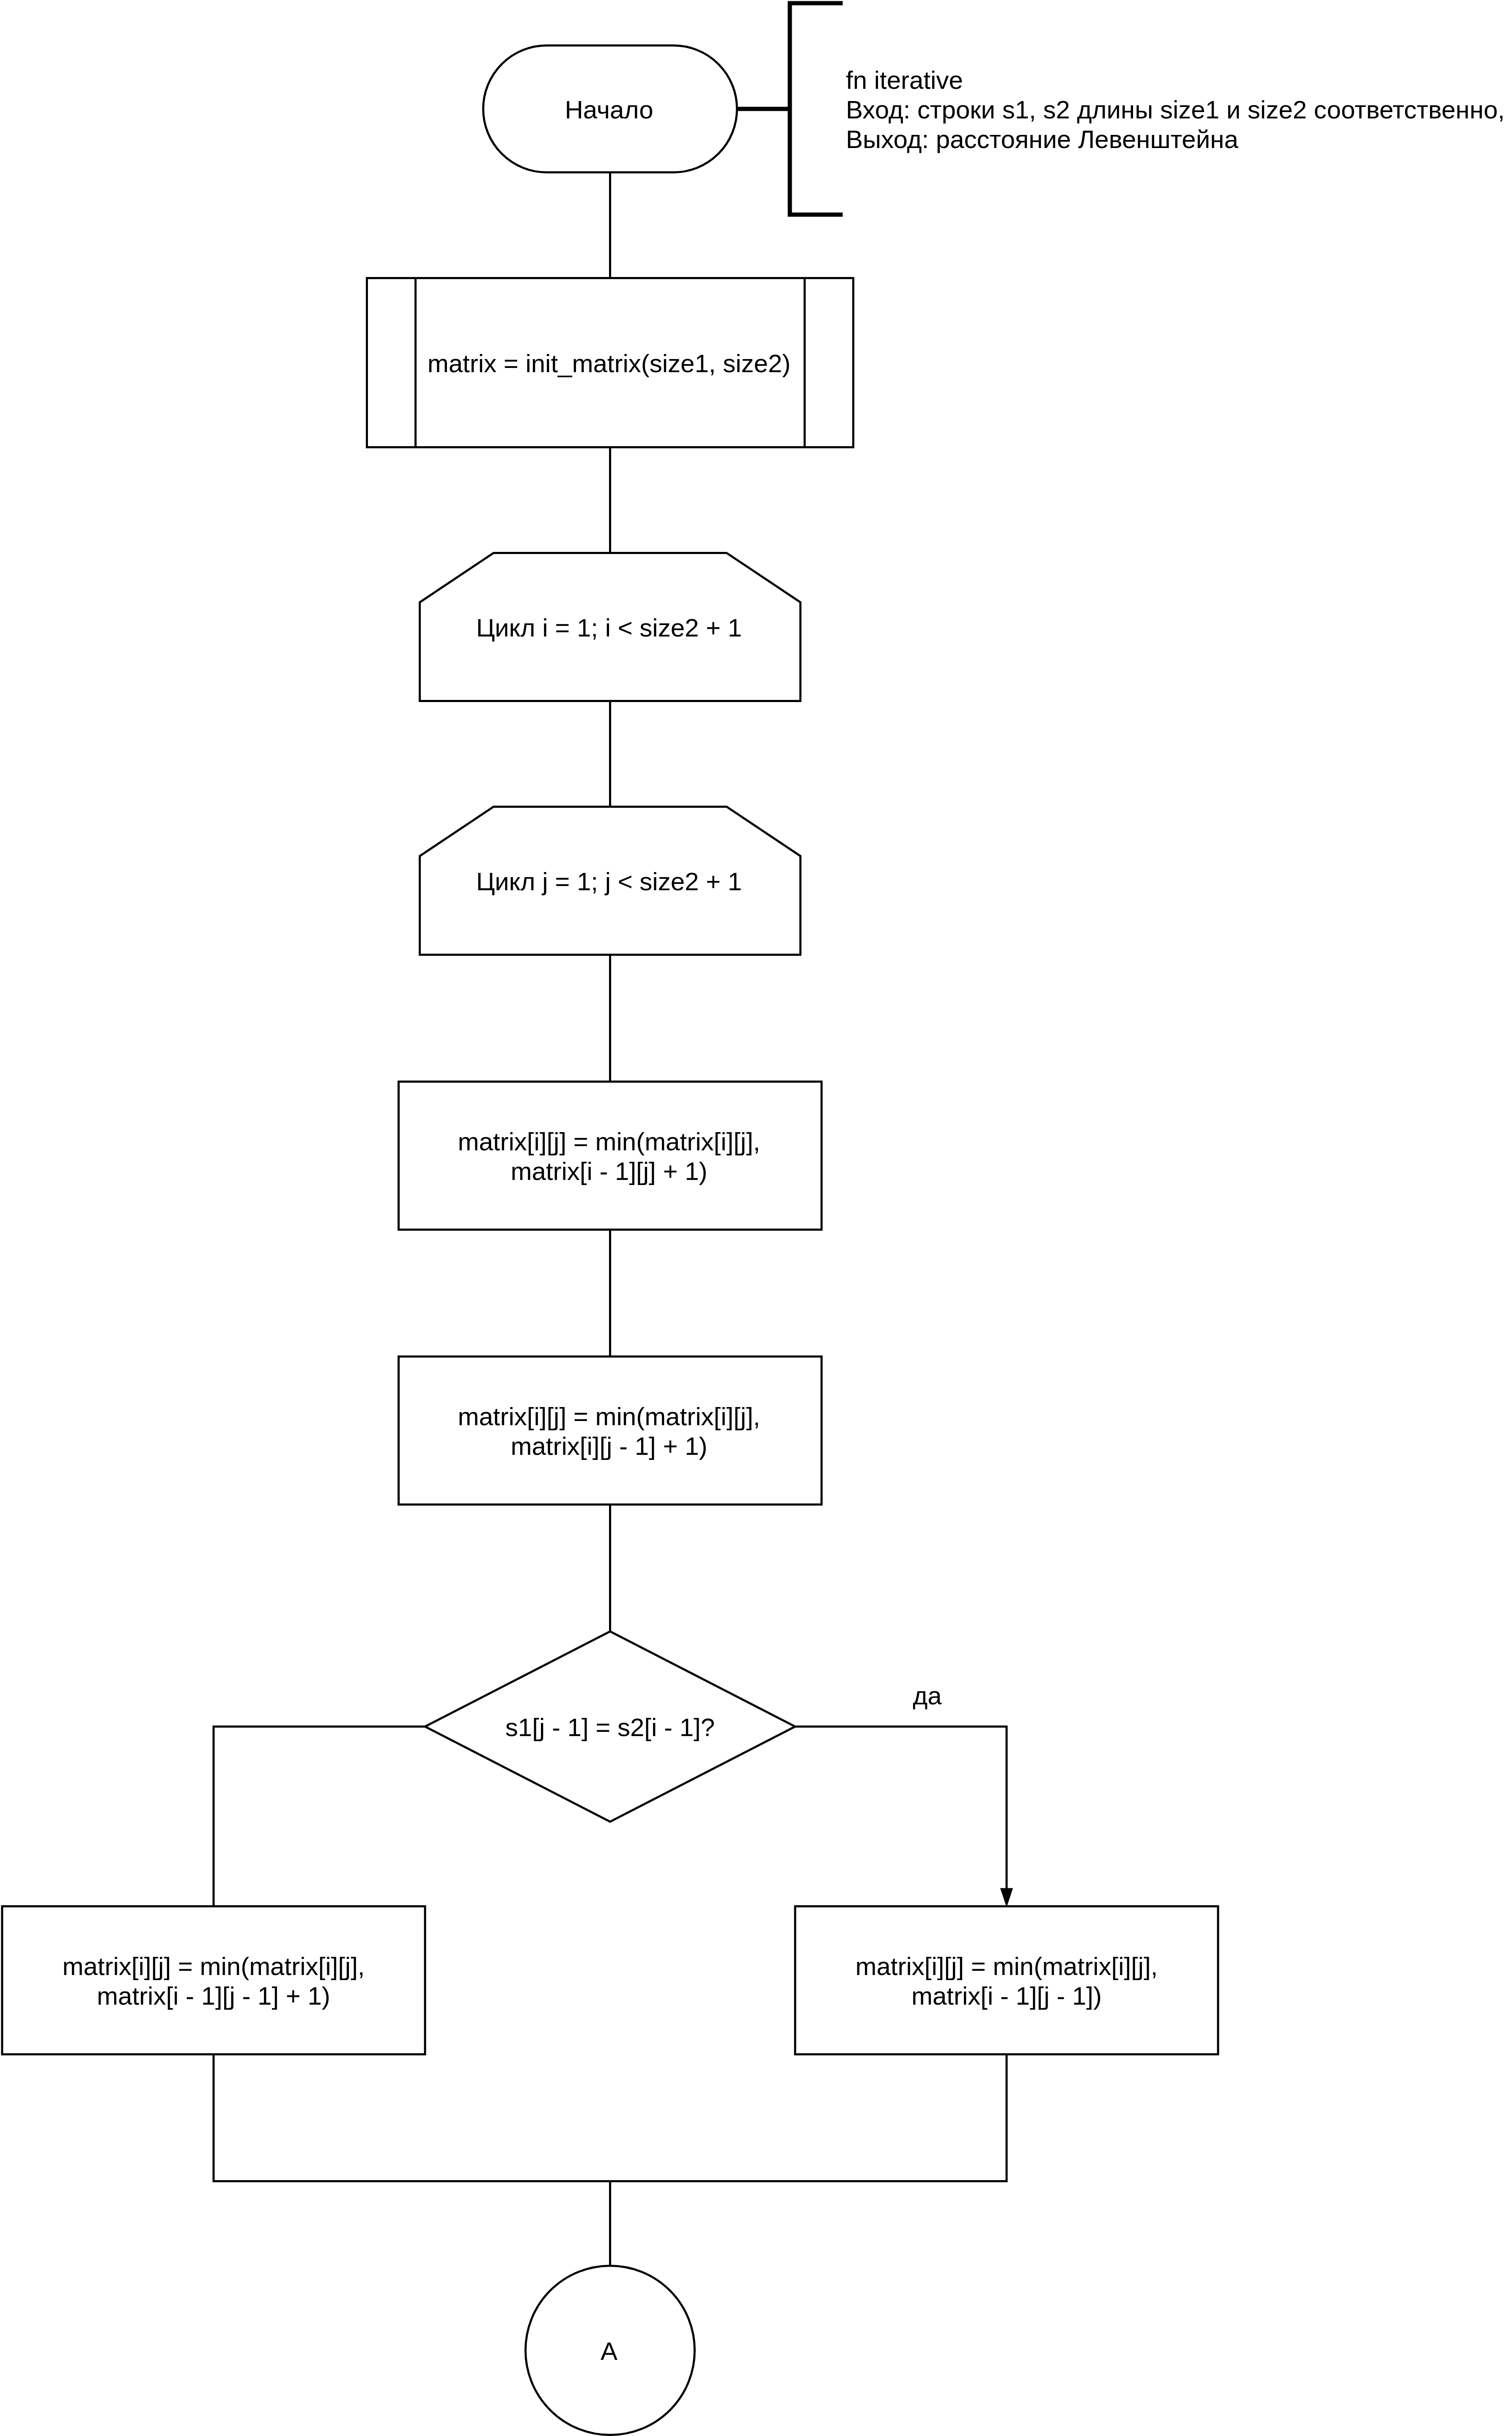
\includegraphics[height=220mm]{iterative_dl}
\caption{Схема итеративного алгоритма нахождения расстояния Дамерау-Левенштейна}
\label{fig:mpr}
\end{figure}

\begin{figure}[h]
\centering
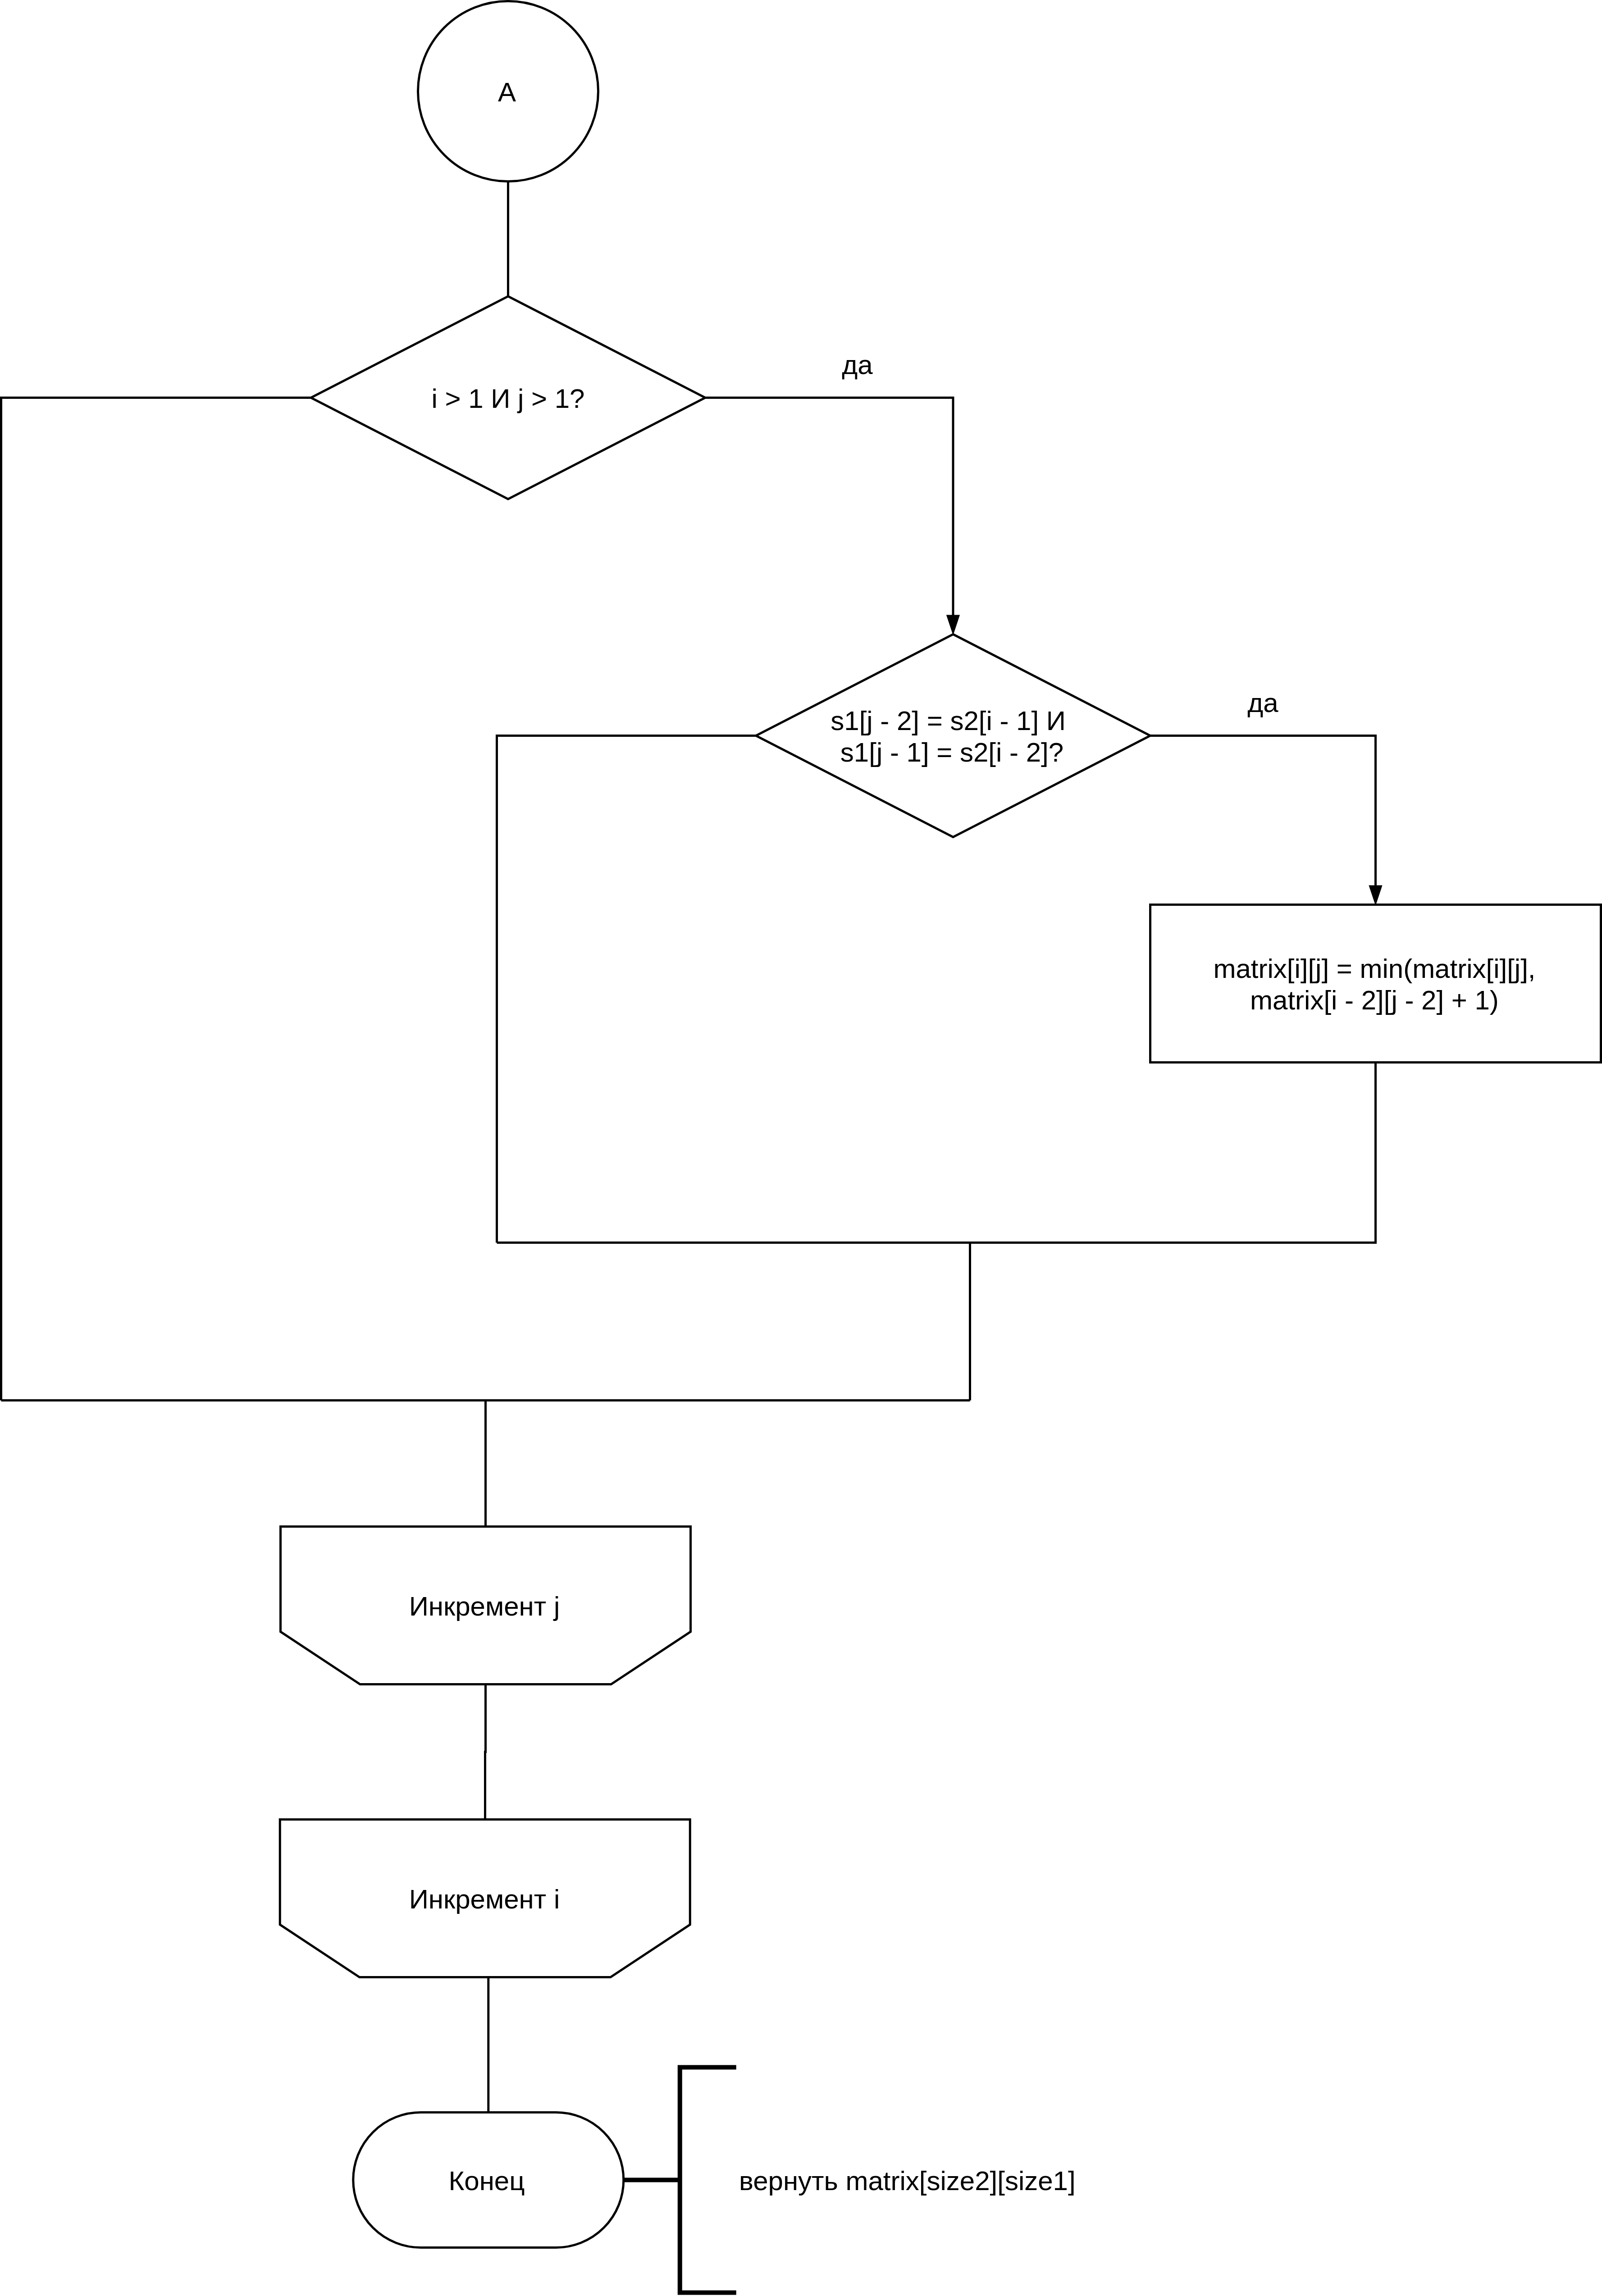
\includegraphics[height=220mm]{iterative_dl_2}
\caption{Продолжение схемы матричного алгоритма нахождения расстояния Дамерау-Левенштейна}
\label{fig:mpr}
\end{figure}
